\documentclass{article}

\usepackage[T1]{fontenc}
\usepackage[utf8]{inputenc}
\usepackage{lmodern}
\usepackage{listings}
\usepackage[colorlinks = true,
            linkcolor = blue,
            urlcolor  = blue,
            citecolor = blue,
            anchorcolor = blue]{hyperref}
\usepackage{graphicx}
\usepackage{subfig}
\usepackage[dvipsnames,table,xcdraw]{xcolor}
\usepackage{array}
\newcolumntype{P}[1]{>{\centering\arraybackslash}p{#1}}
\newcolumntype{M}[1]{>{\centering\arraybackslash}m{#1}}
\author{Francesco Boi}
\title{Self-driving cars program - project  4: Behavioural Cloning}
\date{}

\let\cd\lstinline

\begin{document}
% Python style for highlighting

\maketitle
\tableofcontents 

\lstdefinestyle{customc}{
  belowcaptionskip=1\baselineskip,
  breaklines=true,
  %frame=L,
  xleftmargin=\parindent,
  language = Python,
  showstringspaces=false,
  basicstyle=\footnotesize\ttfamily,
  keywordstyle=\bfseries\color{blue!85!black},
  commentstyle=\itshape\color{gray},
  identifierstyle=\color{black},
  stringstyle=\color{red},
  numbers=left,                    				% where to put the line-numbers; possible values are (none, left, right)
  numbersep=5pt,                   			% how far the line-numbers are from the code
  numberstyle=\tiny\color{gray},     % the style that is used for the line-numbers
  stepnumber=1,
  tabsize=4,
}
\lstdefinestyle{customasm}{
  belowcaptionskip=1\baselineskip,
  frame=L,
  %xleftmargin=\parindent,
  language=[x86masm]Assembler,
  basicstyle=\footnotesize\ttfamily,
  commentstyle=\itshape\color{purple!40!black},
  stepnumber=1,
   tabsize=4,
}
\definecolor{lightgray}{rgb}{.9,.9,.9}
\definecolor{darkgray}{rgb}{.4,.4,.4}
\definecolor{purple}{rgb}{0.65, 0.12, 0.82}
\lstset{escapechar=ç,style=customc}
\section{Content of the project}
Here is the content of the project:
\begin{itemize}
\item \textit{writeup.pdf} (this file): report of the project;
\item \textit{writeup.tex}: source tex file;
\item \textit{model.py}: Python file to train the Convolutional Neural Network;
\item \textit{model.h5}: trained Keras model;
\item \textit{P4Data.tar.gz}: archive containing data to train the model;
\item \textit{P4OtherData.tar.gz}: archive containing additional training data;
\item \textit{drive.py}: Python script to autonomously drive the vehicle on the simulator using the trained neural network and to generate the images for the output video;
\item \textit{run1.tar.gz}: archive containing the images output by \textit{drive.py} to generate the output file;
\item \textit{video.py}: Python script to generate the output video required by the project using the images in \textit{run1.tar.gz};
\item \textit{video.mp4}: output video of the project;
\item \textit{merge\_data.py}: Python script to merge dataset recorded in different training sessions of the simulator;
\item \textit{README.md}: file giving a general description of the project and instructions to set a virtual environment and how to run the script.
\end{itemize}

\section{Project goals}
The steps of this project are the following:
\begin{itemize}
\item use the simulator to collect data of good driving behaviour;
\item build, a convolution neural network in Keras that predicts steering angles from images;
\item train and validate the model with a training and validation set;
\item test that the model successfully drives around track one without leaving the road;
\item summarize the results with a written report.
\end{itemize}

\section{Instruction}
Instructions to run the scripts are given in the README.md file.

\section{Data collection}
Initially both tracks were used to train the model, driving the simulator both clockwise and anti-clockwise. Furthermore, the simulator was driven to recover the centre of the track when offroad. Unfortunately, the huge amount of data meant the training was extremely slow, especially due to the generator use. For this reason, new data were collected by driving the car around the track for three laps only.

\section{Model architecture}
The model architecture is very similar to the Nvidia model with some changes. Particularly, dropout layers  were added to the dense layers with $100$ and $50$ neurons with a dropping probability of $0.25$. No dropout layer was added to the last but one layer with $10$ neurons since it has much less units than the previous layers. Unlike the model in the lectures, all the dense layer except the output one have a ReLU activation function: having multiple dense layers without an activation is equivalent to having a single dense layer due to the linear operations involved. The output layer has no activation: since the steering is between $-1$ and $1$, some experiments were carried out with a $tanh$ but it did not improve the situation.

Here is the final architecture:
\begin{table}
\centering
\scriptsize
\begin{tabular}{ |M{2.2cm}|M{1.55cm}|M{1.55cm}|M{0.75cm}|M{0.59cm}|M{0.71cm}| }
 \hline
 \multicolumn{6}{|c|}{Neural network layers} \\
 \hline
Layer & Input & Output & Stride & Pad & Act.\\
 \hline
Lambda   &(160, 320, 3)&(160, 320, 3)&/&/&/\\
Crop(50, 20, 0, 0)&(160, 320, 3)&(90, 320, 3)&/&/&/\\
Conv2D(5, 5, 24) & (90, 320, 3) & (43, 158, 24)& (2, 2)&def.&relu\\
Conv2D(5, 5, 36) & (43, 158, 24) &(20, 77, 36) & (2, 2)&def.&relu\\
Conv2D(5, 5, 48) &  (20, 77, 36) & (8,37,48)& (2, 2)&def.&relu\\
Conv2D (3, 3, 64) &  (8, 37, 48)& (6, 35, 64) & (1, 1)&def.&relu\\
Conv2D (3, 3, 64) &  (6, 35, 64) & (4,33,64)& (1, 1)&def.&relu\\
Flatten & (4,33,64) &  (8448)&  / &/&relu\\
Dense(100) &(8448) & (100) & / & / & relu\\
Dropout(0.25)& (100) & (100) & / & / & /\\
Dense(50) &(100) & (50) & / & / & relu\\
Dropout(0.25) & (50) & (50) & / & / & /\\
Dense(10) &(50) & (10) & / & / & relu\\
Dense(1) &(10) & (1) & / & / & none\\
\hline
\end{tabular}
\end{table}
\autoref{fig:model} produced with \cd+keras.utils.plot_model+ shows the architecture graphically.
\begin{figure}
\centering
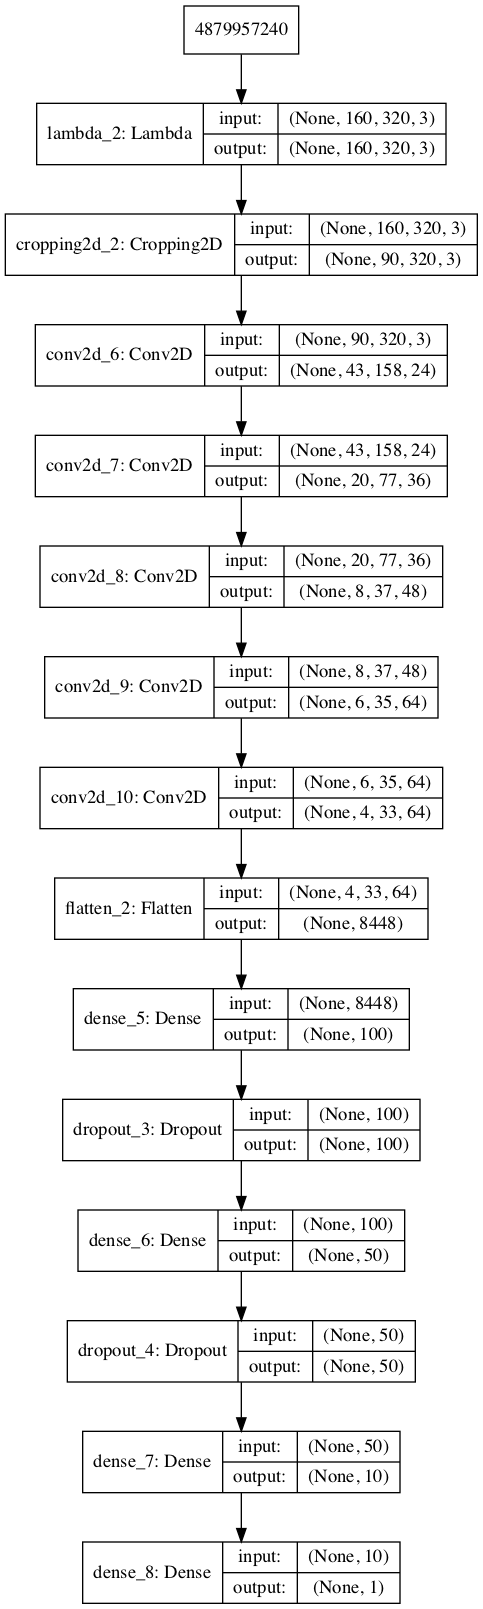
\includegraphics[scale=0.3]{model.png}
\caption{Graphical representation of the model with input and output shapes.}
\label{fig:model}
\end{figure}


\subsection{Lambda layer}
A lambda layer is used to normalize input pixel values within $-0.5$ and $0.5$. 

\subsection{Cropping layer}
The \cd+Cropping2D+ layer crops the input images by $50$ pixels from the top and $20$ from below. These regions of the image are not useful for the steering prediction.

\section{Training}
The model was first trained for 10 epochs. Then, it was retrained for other 5 epochs, obtaining a huge improvement for the autonomous driving. For this reason it was trained for other 5 epochs. With a total of $20$ epochs, the model was finally able to drive around the first track.

To reload the model the keras utility \cd+keras.models.load_model+ was used.

For the training, the centre, left and right images were used. Furthermore, they were also flipped to make up for the overrepresentation of left-turning images. The steering for the flipped images was multiplied by $-1$. For the left and right cameras images, the correction factor was set to $0.4$.

The images were shuffled by the generator before being used for the training process.

\subsection{Optimizer}
The learning rate optimizer was set to $0.001$, which is equal to default one. Some experiments with smaller learning rates and an adaptive one were carried out but it was difficult to see any improvement in the model.

\subsection{Loss}
The chosen loss is the MSE.

\subsection{Batch size}
The batch size was set to $32$. Bigger batch sizes were tested with not-so-good results and slower convergence.

\end{document}